% This is "sig-alternate.tex" V2.1 April 2013
% This file should be compiled with V2.5 of "sig-alternate.cls" May 2012
%
% This example file demonstrates the use of the 'sig-alternate.cls'
% V2.5 LaTeX2e document class file. It is for those submitting
% articles to ACM Conference Proceedings WHO DO NOT WISH TO
% STRICTLY ADHERE TO THE SIGS (PUBS-BOARD-ENDORSED) STYLE.
% The 'sig-alternate.cls' file will produce a similar-looking,
% albeit, 'tighter' paper resulting in, invariably, fewer pages.
%
% ----------------------------------------------------------------------------------------------------------------
% This .tex file (and associated .cls V2.5) produces:
%       1) The Permission Statement
%       2) The Conference (location) Info information
%       3) The Copyright Line with ACM data
%       4) NO page numbers
%
% as against the acm_proc_article-sp.cls file which
% DOES NOT produce 1) thru' 3) above.
%
% Using 'sig-alternate.cls' you have control, however, from within
% the source .tex file, over both the CopyrightYear
% (defaulted to 200X) and the ACM Copyright Data
% (defaulted to X-XXXXX-XX-X/XX/XX).
% e.g.
% \CopyrightYear{2007} will cause 2007 to appear in the copyright line.
% \crdata{0-12345-67-8/90/12} will cause 0-12345-67-8/90/12 to appear in the copyright line.
%
% ---------------------------------------------------------------------------------------------------------------
% This .tex source is an example which *does* use
% the .bib file (from which the .bbl file % is produced).
% REMEMBER HOWEVER: After having produced the .bbl file,
% and prior to final submission, you *NEED* to 'insert'
% your .bbl file into your source .tex file so as to provide
% ONE 'self-contained' source file.
%
% ================= IF YOU HAVE QUESTIONS =======================
% Questions regarding the SIGS styles, SIGS policies and
% procedures, Conferences etc. should be sent to
% Adrienne Griscti (griscti@acm.org)
%
% Technical questions _only_ to
% Gerald Murray (murray@hq.acm.org)
% ===============================================================
%
% For tracking purposes - this is V2.0 - May 2012

\documentclass{sig-alternate-05-2015}


\begin{document}

% Copyright
\setcopyright{acmcopyright}
%\setcopyright{acmlicensed}
%\setcopyright{rightsretained}
%\setcopyright{usgov}
%\setcopyright{usgovmixed}
%\setcopyright{cagov}
%\setcopyright{cagovmixed}


% DOI
\doi{10.475/123_4}

% ISBN
\isbn{123-4567-24-567/08/06}

%Conference
\conferenceinfo{CS838 Fall 2016}{University of Wisconsin-Madison}

\acmPrice{\$15.00}

%
% --- Author Metadata here ---
\conferenceinfo{WOODSTOCK}{'97 El Paso, Texas USA}
%\CopyrightYear{2007} % Allows default copyright year (20XX) to be over-ridden - IF NEED BE.
%\crdata{0-12345-67-8/90/01}  % Allows default copyright data (0-89791-88-6/97/05) to be over-ridden - IF NEED BE.
% --- End of Author Metadata ---

\title{Measuring and Improvig Geo Distributed Storage}
\subtitle{CS838 Fall 2016 Project Report}
%
% You need the command \numberofauthors to handle the 'placement
% and alignment' of the authors beneath the title.
%
% For aesthetic reasons, we recommend 'three authors at a time'
% i.e. three 'name/affiliation blocks' be placed beneath the title.
%
% NOTE: You are NOT restricted in how many 'rows' of
% "name/affiliations" may appear. We just ask that you restrict
% the number of 'columns' to three.
%
% Because of the available 'opening page real-estate'
% we ask you to refrain from putting more than six authors
% (two rows with three columns) beneath the article title.
% More than six makes the first-page appear very cluttered indeed.
%
% Use the \alignauthor commands to handle the names
% and affiliations for an 'aesthetic maximum' of six authors.
% Add names, affiliations, addresses for
% the seventh etc. author(s) as the argument for the
% \additionalauthors command.
% These 'additional authors' will be output/set for you
% without further effort on your part as the last section in
% the body of your article BEFORE References or any Appendices.

\numberofauthors{8} %  in this sample file, there are a *total*
% of EIGHT authors. SIX appear on the 'first-page' (for formatting
% reasons) and the remaining two appear in the \additionalauthors section.
%
\author{
% You can go ahead and credit any number of authors here,
% e.g. one 'row of three' or two rows (consisting of one row of three
% and a second row of one, two or three).
%
% The command \alignauthor (no curly braces needed) should
% precede each author name, affiliation/snail-mail address and
% e-mail address. Additionally, tag each line of
% affiliation/address with \affaddr, and tag the
% e-mail address with \email.
%
% 1st. author
\alignauthor
Karan Bavishi \\
       \affaddr{UW Madison}\\
% 2nd. author
\alignauthor
Hasnain Ali Pirzada\\
\affaddr{UW Madison}\\
% 3rd. author
}
% There's nothing stopping you putting the seventh, eighth, etc.
% author on the opening page (as the 'third row') but we ask,
% for aesthetic reasons that you place these 'additional authors'
% in the \additional authors block, viz.
% Just remember to make sure that the TOTAL number of authors
% is the number that will appear on the first page PLUS the
% number that will appear in the \additionalauthors section.

\maketitle
\section{Problem Statement}
HDFS and other distributed file systems are designed to work in a single data center and do not scale well to a geo distributed environment. The primary reason for this is the heterogeneity of the the inter and intra datacenter links and the fact that the file system itself is unaware of the thin links that connect multiple geo locations. One major way to overcome these problems is to use Erasure Coding instead of replication since erasure coding produces much less amount of data compared to replication and as a result the network and storage overheads are reduced. To solve these problems our goal in this project was two fold. Our first target was to quantify and analyse the performance degradation of HDFS (both replication and erasure coding based) running geo distributedly. Depending upon our findings of this, our second major goal was to reduce the impact of thin WAN links on the performance of geo distributed HDFS. We achieved these goals by first benchmarking both HDFS and HDFS Erasure Coding (HDFS-EC) running geo distributedly and compared their performance with the same system running in a single datacenter. In the second phase of the project we modified HDFS-EC and used greedy heuristics to make it WAN aware while performing both reads and writes.

%
% The code below should be generated by the tool at
% http://dl.acm.org/ccs.cfm
% Please copy and paste the code instead of the example below. 
%





%
% End generated code
%

%
%  Use this command to print the description
%
\printccsdesc

% We no longer use \terms command
%\terms{Theory}

\keywords{HDFS; Erasure Coding; Geo Distributed Storage}

\section{System Set up}
The first part of our project was to quantify the degradation in HDFS and HDFS-EC performance in Geo Distributed (GD) settings. To do this, we set up a cluster of machines placed in different geo locations , with HDFS running on top of them. We needed to chose the number of machines and the replication factor in such a way that at least one replica is guaranteed to be on a datanode in another DC so that the WAN links are brought into play. 

To be able to measure the extent of degradation in GD settings we also needed to run the same set of experiments in a non GD environment. Furthermore, to be able to compare the extent of degradation in replication based scheme vs the erasure coding scheme we needed to run the same set of experiments on HDFS with replication as well as HDFS-EC in both GD and non GD environment. So in total we had four different settings which are described and explained as follows:

\begin{enumerate}
  \item \textbf{HDFS-Replication based} HDFS running with replication factor 3 with three datanodes in Wisc CloudLab. This is the base case for measuring  and compare the GD degradation in replication based HDFS. There is no remote node since there is just one datacenter.  
	\item \textbf{HDFS-Replica-GD} HDFS running with replication factor 3 with two datanodes in Wisc CloudLab and one datanode in Clemson. A replication factor of 3 here with 2 datanodes in Wisconsin and 1 in Clemson ensure that one replica of each block is located remotely.
	\item \textbf{HDFS-EC} HDFS running with erasure coding scheme Reed-Solomon (3,2) with five datanodes in Wisc CloudLab. HDFS-EC fork that we used required at least n + r datanodes in the cluster while using  RS(n,r) erasure coding scheme. This is done to ensure that stripes cells are well distributed across the cluster since the number of failures that can be tolerated here is equal to r i.e., 2 in this case. A good distribution of the stripe cells ensures better fault tolerance.  Hence, for this configuration we require 3 + 2 = 5 datanodes. All of them are in Wiscnosin.
	\item \textbf{HDFS-EC-GD} HDFS running with erasure coding scheme Reed-Solomon (3,2) with four datanodes in Wisc CloudLab and one datanode in Clemson. The reason for choosing 5 nodes in total is same as the above one. However, now four of the five datanodes are in Wisconsin and one is in Clemson forcing every write to involve the WAN. 
  \end{enumerate}
The WAN speed for all the above configurations is measure to be around 1 Gbps while the intra DC links are all 10 Gbps. This high difference in the two link speeds allows us to more realistically observe the effect of WAN link degradation. We rigorously evaluated all the HDFS variants described using the TestDFSIO workloads. The details are in the experiments and results section. 

\section{System Design \& Implementation}
Drawing insights from the results (which we describe and explain in the results section) of our performance benchmarking of HDFS in GD settings (both replicationa and EC based)  we implemented WAN awareness in HDFS-EC and tuned both the read and write pipelines to take WAN into account while deciding on the datanodes for read/write for the HDFS client. 
\subsection{WAN awareness for HDFS-EC Reads}
Let us say we have a file stored in HDFS-EC running atop a cluster which has nodes in two datacenters A and B. The file is stored as a stripe of cells (a picture here maybe?) with some cells representing actual data and others representing parity. Further assume that the file has 3 cells of data which would result in a total of 5 cells written in HDFS 3 being the data cells and 2 being the parity cells. Assume that datacenter A has 2 data cell and one parity cell, while datacenter B has 1 data cell and one parity cell. Now, there HDFS-EC client in datacenter A who wants to read a file.  The default policy is to read all the data cells. The parity cells are only read when the data cell is unavailable because of the high computation cost of reconstructing the data from parity.


In a single data center circumstances, this makes sense because the computation cost is very likely to exceed the network cost that is paid to read a data cells from a remote node.  However, in a GD cluster, this may not be true. So in this case, depending upon the current WAN cost it might be faster to actually read 2 data cells and 1 parity cell locally and reconstruct all the three datacells in datacenter A.

To achieve this, we associate costs with both the computation of the data cell and reading it over the WAN and the client greedily chooses the whichever one has the lower cost. We start with simple static costs for the WAN links and computation which we hard code at the beginning. However, both of these can be made a function of current cpu load of the client and the current WAN load.

\subsection{WAN awareness for HDFS-EC Writes Using Greedy Heuristic}
The write policy in HDFS-EC is similar. The namenode selects (r + s) nodes for writing r data cells and the corresponding s parity cells. It then writes these cells in round robin way to all these datanodes. This is done to avoid the loss of multiple data cells in case of a datanode failure. However, while choosing the datanodes to store data and parity cells, the namenode can select a datanode in the other datacenter despite having a datanode locally. This would involve the the write to go through a WAN. 

To prevent this situation, we again implement a simple cost model in the HDFS-EC write pipeline. We associate a parameter same-rack-penalty with every write. Moreover, we have link costs available between every pair of racks in the topology. Whenever an HDFS-EC client wants to write a file, the namenode sorts the available datanodes according to their distance from the writer. Now, for each block to be written, it picks the datanode with the minimum cost and remembers the rack from which this datanode was picked. When choosing a datanode for the next block to be written it picks the datanode with the minimum cost with the added constraint that if another datanode has already been chosen from the same rack the total cost of this node becomes y and if this total cost is still the minimum of the cost of all the available data nodes this  datanode is chosen. Now, for any subsequent iterations, the cost of this datanode would be (linkcost + n * samerackpenalty) where n is the number of times a datanode from this rack has been chosen for this client. 

\textbf{How does this scheme help?}

This method of selecting the datanodes for writes has a direct affect on the WAN usage. Since the cost of any datanode in datacenter B is always much higher, the namenode will select the write locations which are closer to the writer reducing the WAN usage. A side effect of this would be that the data would be aggregated near the producers.  For large enough files however, the datanodes in the remote datacenter would eventually be selected since penalty for a given rack increases linearly with the number of blocks that have already been written in the same rack so at some point selecting a rack in the same datacenter would have more cost than writing to the remote one. 

\section{Experiments \& Results}

Our experiments and results for this project are divided into two parts. In the first part we describe and explain the the benchmarking experiments we performed to measure the degradation of performance of HDFS and HDFS-EC in GD settings. In the second part we discuss the results of our WAN aware HDFS-EC. 

\section{Discussion}

\subsection{Erasure Coding Properties and their effect}

There are various kinds of encoding families that can be used to encode data. These include RS codes, LRC codes and the product codes. Since HDFS-EC used RS encoding we will restrict our discussion to tradeoffs of using different values k and r in RS encoding. According to the coding theory a (k, r) RS code entails the minimum storage overhead among all (k, r) erasure codes that tolerate any r failures [cite hitchhiker]. Moreover, RS codes can be constructed with arbitrary values of k and r depending upon the system at hand [cite hitchiker]. These two properties make RS codes very attractive for use in large scale storage systems. 


The choice of the parameters k and r for any particular system determines the storage overhead and recovery cost for the system. In general achieving lower storage overhead increases the recovery cost of the system and vice versa. For Example, an RS(10, 4) system has a 1.4x overhead compared to 1.5x for RS (6, 3). However, in case of an unavailable datablock RS (10, 4) has to read 10 blocks while RS (6, 3) only needs to read 6.This trend can be generalized for any possible values or k and r. 



\subsection{Significance of Storage Unit to Encode}

The storage unit to be encoded is determined by the layout of the file system. This layout can be contiguous or striped. In contiguous layout a logical block of the file system is mapped directly to a datanode. Reading that block merely involves contacting that particular datanode and doing one I/O.  In striped block layout however, a single logical block in the file system is broken down into small cells and these cells are then mapped to the available datanodes in a round robin manner. Therefore, in the striped layout case, reading a single logical datablock of the file system involves doing I/O with all the datanodes that store the cells of that block. 

%This however, may not be very suitable for Map-Reduce style applications because data %locality cannot be achieved as most reads would involve multiple remote I/Os.

In the replication based storage, a contiguous layout seems to be an obvious choice as there is no point in paying an extra cost of many remote reads for every read event. However, in Erasure Coded storage, things become a little more interesting. This is because the number of parity blocks computed in RS encoding scheme is always equal to r irrespective of the total number of data blocks in the file [cite blog]. For example, while using RS (10, 4) if a file consists of just one data block, it will still end up computing and writing 4 parity blocks resulting in a total storage overhead of 400\% which is worse than 3x replication! However, in a striped layout and assuming a cell size of 1 MB and the HDFS data block size of 128MB the same 1 block file would still have a 1.4 x overhead since it will produce about 51 MBs of parity (since the parity is computed for 1 MB stripe cells) compared to 512 MB of parity produced by the contiguous layout for the same 128 MB file. 

Therefore, the type of file system layout directly affects the storage overhead for the erasure coding scheme at hand. This choice of layout in turn is determined the file size distribution on the cluster. Hence, a cluster with many small files is not suitable for erasure coding in the contiguous layout because the storage overhead would be worse than replication. The HDFS-EC alpha release that we used and extended uses a striped layout with 1 MB cell size. 



%\subsection{Type Changes and {\subsecit Special} Characters}
%We have already seen several typeface changes in this sample.  You
%can indicate italicized words or phrases in your text with
%the command \texttt{{\char'134}textit}; emboldening with the
%command \texttt{{\char'134}textbf}
%and typewriter-style (for instance, for computer code) with
%\texttt{{\char'134}texttt}.  But remember, you do not
%have to indicate typestyle changes when such changes are
%part of the \textit{structural} elements of your
%article; for instance, the heading of this subsection will
%be in a sans serif\footnote{A third footnote, here.
%Let's make this a rather short one to
%see how it looks.} typeface, but that is handled by the
%document class file. Take care with the use
%of\footnote{A fourth, and last, footnote.}
%the curly braces in typeface changes; they mark
%the beginning and end of
%the text that is to be in the different typeface.
%
%You can use whatever symbols, accented characters, or
%non-English characters you need anywhere in your document;
%you can find a complete list of what is
%available in the \textit{\LaTeX\
%User's Guide}\cite{Lamport:LaTeX}.
%
%\subsection{Math Equations}
%You may want to display math equations in three distinct styles:
%inline, numbered or non-numbered display.  Each of
%the three are discussed in the next sections.
%
%\subsubsection{Inline (In-text) Equations}
%A formula that appears in the running text is called an
%inline or in-text formula.  It is produced by the
%\textbf{math} environment, which can be
%invoked with the usual \texttt{{\char'134}begin. . .{\char'134}end}
%construction or with the short form \texttt{\$. . .\$}. You
%can use any of the symbols and structures,
%from $\alpha$ to $\omega$, available in
%\LaTeX\cite{Lamport:LaTeX}; this section will simply show a
%few examples of in-text equations in context. Notice how
%this equation: \begin{math}\lim_{n\rightarrow \infty}x=0\end{math},
%set here in in-line math style, looks slightly different when
%set in display style.  (See next section).
%
%\subsubsection{Display Equations}
%A numbered display equation -- one set off by vertical space
%from the text and centered horizontally -- is produced
%by the \textbf{equation} environment. An unnumbered display
%equation is produced by the \textbf{displaymath} environment.
%
%Again, in either environment, you can use any of the symbols
%and structures available in \LaTeX; this section will just
%give a couple of examples of display equations in context.
%First, consider the equation, shown as an inline equation above:
%\begin{equation}\lim_{n\rightarrow \infty}x=0\end{equation}
%Notice how it is formatted somewhat differently in
%the \textbf{displaymath}
%environment.  Now, we'll enter an unnumbered equation:
%\begin{displaymath}\sum_{i=0}^{\infty} x + 1\end{displaymath}
%and follow it with another numbered equation:
%\begin{equation}\sum_{i=0}^{\infty}x_i=\int_{0}^{\pi+2} f\end{equation}
%just to demonstrate \LaTeX's able handling of numbering.
%
%\subsection{Citations}
%Citations to articles \cite{bowman:reasoning,
%clark:pct, braams:babel, herlihy:methodology},
%conference proceedings \cite{clark:pct} or
%books \cite{salas:calculus, Lamport:LaTeX} listed
%in the Bibliography section of your
%article will occur throughout the text of your article.
%You should use BibTeX to automatically produce this bibliography;
%you simply need to insert one of several citation commands with
%a key of the item cited in the proper location in
%the \texttt{.tex} file \cite{Lamport:LaTeX}.
%The key is a short reference you invent to uniquely
%identify each work; in this sample document, the key is
%the first author's surname and a
%word from the title.  This identifying key is included
%with each item in the \texttt{.bib} file for your article.
%
%The details of the construction of the \texttt{.bib} file
%are beyond the scope of this sample document, but more
%information can be found in the \textit{Author's Guide},
%and exhaustive details in the \textit{\LaTeX\ User's
%Guide}\cite{Lamport:LaTeX}.
%
%This article shows only the plainest form
%of the citation command, using \texttt{{\char'134}cite}.
%This is what is stipulated in the SIGS style specifications.
%No other citation format is endorsed or supported.
%
%\subsection{Tables}
%Because tables cannot be split across pages, the best
%placement for them is typically the top of the page
%nearest their initial cite.  To
%ensure this proper ``floating'' placement of tables, use the
%environment \textbf{table} to enclose the table's contents and
%the table caption.  The contents of the table itself must go
%in the \textbf{tabular} environment, to
%be aligned properly in rows and columns, with the desired
%horizontal and vertical rules.  Again, detailed instructions
%on \textbf{tabular} material
%is found in the \textit{\LaTeX\ User's Guide}.
%
%Immediately following this sentence is the point at which
%Table 1 is included in the input file; compare the
%placement of the table here with the table in the printed
%dvi output of this document.
%
%\begin{table}
%\centering
%\caption{Frequency of Special Characters}
%\begin{tabular}{|c|c|l|} \hline
%Non-English or Math&Frequency&Comments\\ \hline
%\O & 1 in 1,000& For Swedish names\\ \hline
%$\pi$ & 1 in 5& Common in math\\ \hline
%\$ & 4 in 5 & Used in business\\ \hline
%$\Psi^2_1$ & 1 in 40,000& Unexplained usage\\
%\hline\end{tabular}
%\end{table}
%
%To set a wider table, which takes up the whole width of
%the page's live area, use the environment
%\textbf{table*} to enclose the table's contents and
%the table caption.  As with a single-column table, this wide
%table will ``float" to a location deemed more desirable.
%Immediately following this sentence is the point at which
%Table 2 is included in the input file; again, it is
%instructive to compare the placement of the
%table here with the table in the printed dvi
%output of this document.
%
%
%\begin{table*}
%\centering
%\caption{Some Typical Commands}
%\begin{tabular}{|c|c|l|} \hline
%Command&A Number&Comments\\ \hline
%\texttt{{\char'134}alignauthor} & 100& Author alignment\\ \hline
%\texttt{{\char'134}numberofauthors}& 200& Author enumeration\\ \hline
%\texttt{{\char'134}table}& 300 & For tables\\ \hline
%\texttt{{\char'134}table*}& 400& For wider tables\\ \hline\end{tabular}
%\end{table*}
%% end the environment with {table*}, NOTE not {table}!
%
%\subsection{Figures}
%Like tables, figures cannot be split across pages; the
%best placement for them
%is typically the top or the bottom of the page nearest
%their initial cite.  To ensure this proper ``floating'' placement
%of figures, use the environment
%\textbf{figure} to enclose the figure and its caption.
%
%This sample document contains examples of \textbf{.eps} files to be
%displayable with \LaTeX.  If you work with pdf\LaTeX, use files in the
%\textbf{.pdf} format.  Note that most modern \TeX\ system will convert
%\textbf{.eps} to \textbf{.pdf} for you on the fly.  More details on
%each of these is found in the \textit{Author's Guide}.
%
%\begin{figure}
%\centering
%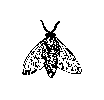
\includegraphics{fly}
%\caption{A sample black and white graphic.}
%\end{figure}
%
%\begin{figure}
%\centering
%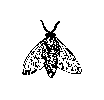
\includegraphics[height=1in, width=1in]{fly}
%\caption{A sample black and white graphic
%that has been resized with the \texttt{includegraphics} command.}
%\end{figure}
%
%
%As was the case with tables, you may want a figure
%that spans two columns.  To do this, and still to
%ensure proper ``floating'' placement of tables, use the environment
%\textbf{figure*} to enclose the figure and its caption.
%and don't forget to end the environment with
%{figure*}, not {figure}!
%
%\begin{figure*}
%\centering
%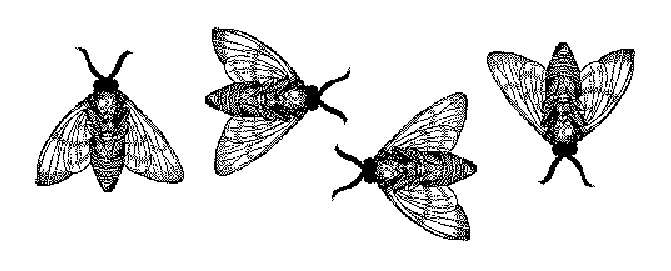
\includegraphics{flies}
%\caption{A sample black and white graphic
%that needs to span two columns of text.}
%\end{figure*}
%
%
%\begin{figure}
%\centering
%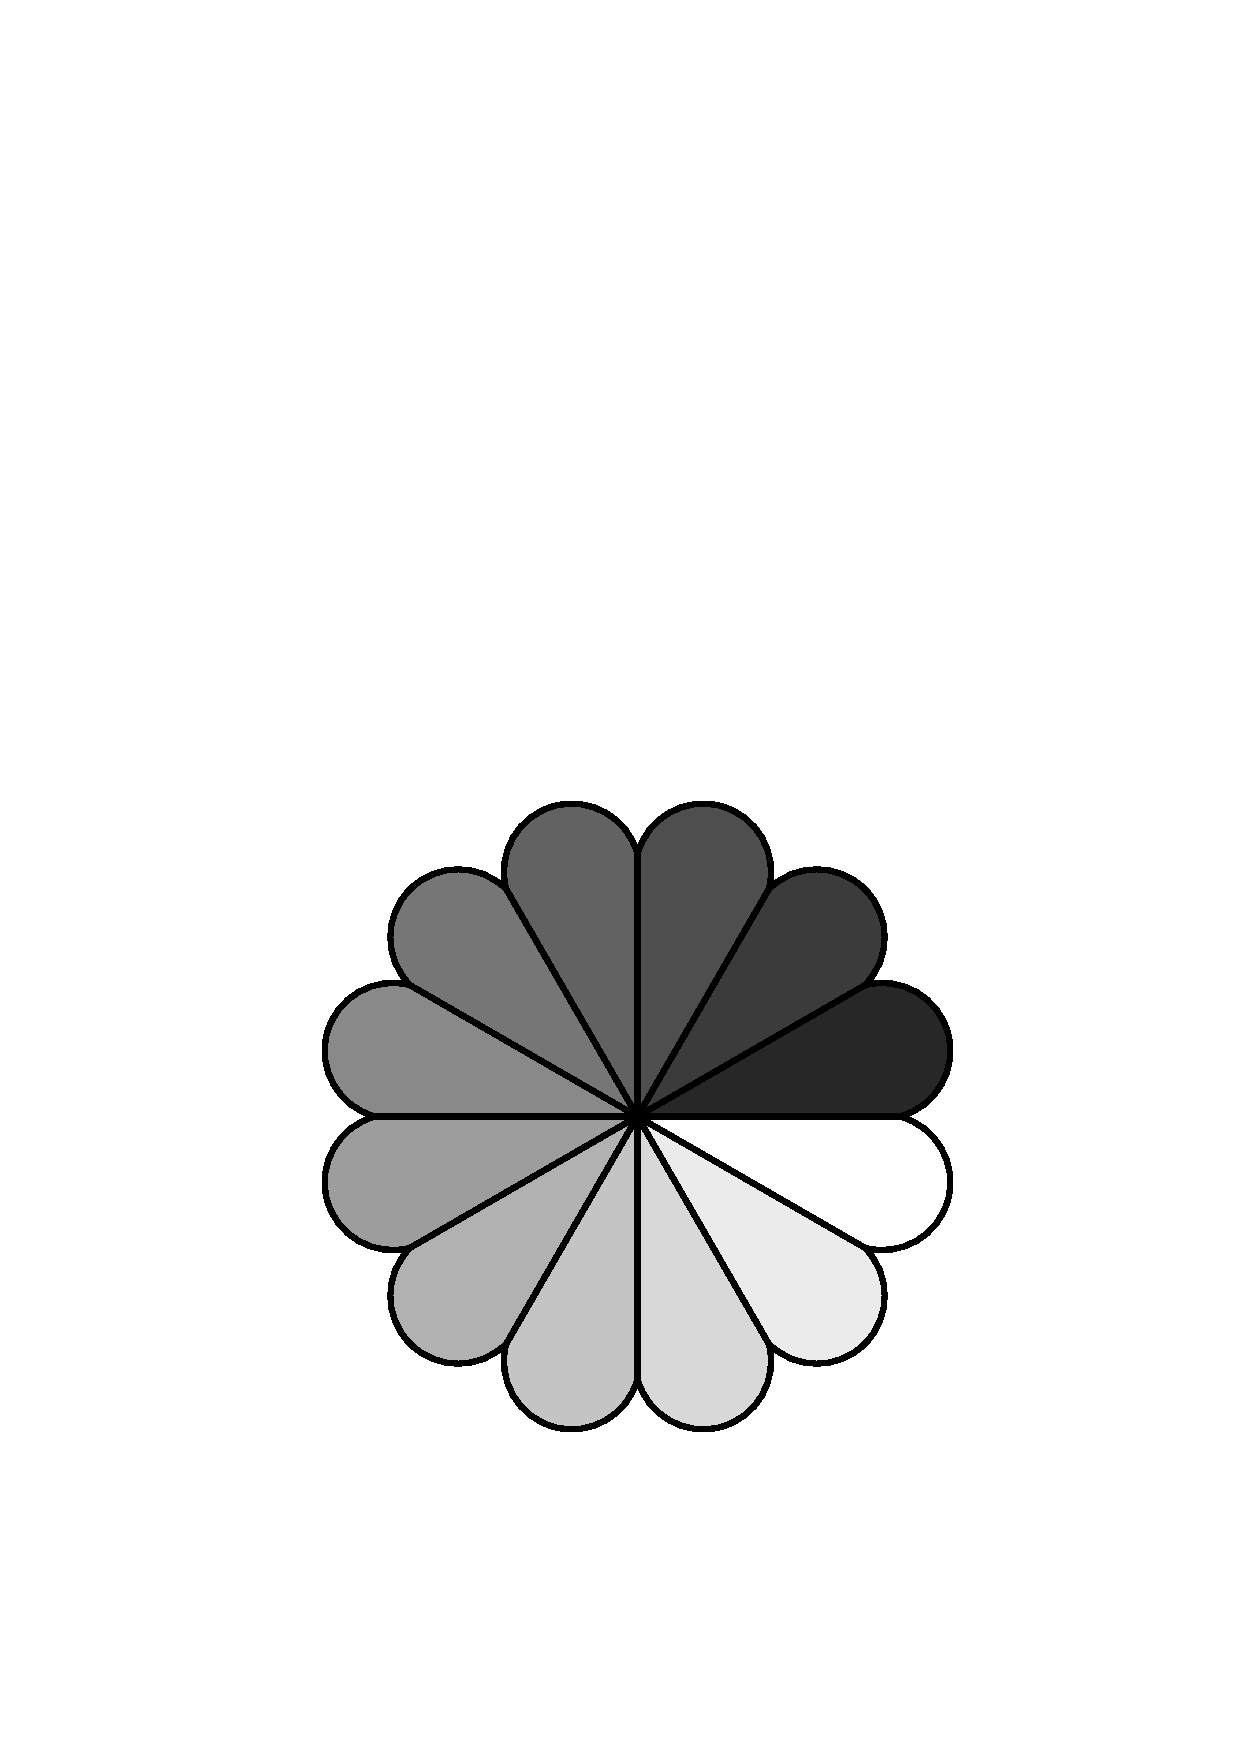
\includegraphics[height=1in, width=1in]{rosette}
%\caption{A sample black and white graphic that has
%been resized with the \texttt{includegraphics} command.}
%\vskip -6pt
%\end{figure}
%
%\subsection{Theorem-like Constructs}
%Other common constructs that may occur in your article are
%the forms for logical constructs like theorems, axioms,
%corollaries and proofs.  There are
%two forms, one produced by the
%command \texttt{{\char'134}newtheorem} and the
%other by the command \texttt{{\char'134}newdef}; perhaps
%the clearest and easiest way to distinguish them is
%to compare the two in the output of this sample document:
%
%This uses the \textbf{theorem} environment, created by
%the\linebreak\texttt{{\char'134}newtheorem} command:
%\newtheorem{theorem}{Theorem}
%\begin{theorem}
%Let $f$ be continuous on $[a,b]$.  If $G$ is
%an antiderivative for $f$ on $[a,b]$, then
%\begin{displaymath}\int^b_af(t)dt = G(b) - G(a).\end{displaymath}
%\end{theorem}
%
%The other uses the \textbf{definition} environment, created
%by the \texttt{{\char'134}newdef} command:
%\newdef{definition}{Definition}
%\begin{definition}
%If $z$ is irrational, then by $e^z$ we mean the
%unique number which has
%logarithm $z$: \begin{displaymath}{\log e^z = z}\end{displaymath}
%\end{definition}
%
%Two lists of constructs that use one of these
%forms is given in the
%\textit{Author's  Guidelines}.
% 
%There is one other similar construct environment, which is
%already set up
%for you; i.e. you must \textit{not} use
%a \texttt{{\char'134}newdef} command to
%create it: the \textbf{proof} environment.  Here
%is a example of its use:
%\begin{proof}
%Suppose on the contrary there exists a real number $L$ such that
%\begin{displaymath}
%\lim_{x\rightarrow\infty} \frac{f(x)}{g(x)} = L.
%\end{displaymath}
%Then
%\begin{displaymath}
%l=\lim_{x\rightarrow c} f(x)
%= \lim_{x\rightarrow c}
%\left[ g{x} \cdot \frac{f(x)}{g(x)} \right ]
%= \lim_{x\rightarrow c} g(x) \cdot \lim_{x\rightarrow c}
%\frac{f(x)}{g(x)} = 0\cdot L = 0,
%\end{displaymath}
%which contradicts our assumption that $l\neq 0$.
%\end{proof}
%
%Complete rules about using these environments and using the
%two different creation commands are in the
%\textit{Author's Guide}; please consult it for more
%detailed instructions.  If you need to use another construct,
%not listed therein, which you want to have the same
%formatting as the Theorem
%or the Definition\cite{salas:calculus} shown above,
%use the \texttt{{\char'134}newtheorem} or the
%\texttt{{\char'134}newdef} command,
%respectively, to create it.
%
%\subsection*{A {\secit Caveat} for the \TeX\ Expert}
%Because you have just been given permission to
%use the \texttt{{\char'134}newdef} command to create a
%new form, you might think you can
%use \TeX's \texttt{{\char'134}def} to create a
%new command: \textit{Please refrain from doing this!}
%Remember that your \LaTeX\ source code is primarily intended
%to create camera-ready copy, but may be converted
%to other forms -- e.g. HTML. If you inadvertently omit
%some or all of the \texttt{{\char'134}def}s recompilation will
%be, to say the least, problematic.
%
%\section{Conclusions}
%This paragraph will end the body of this sample document.
%Remember that you might still have Acknowledgments or
%Appendices; brief samples of these
%follow.  There is still the Bibliography to deal with; and
%we will make a disclaimer about that here: with the exception
%of the reference to the \LaTeX\ book, the citations in
%this paper are to articles which have nothing to
%do with the present subject and are used as
%examples only.
%%\end{document}  % This is where a 'short' article might terminate
%
%%ACKNOWLEDGMENTS are optional
%\section{Acknowledgments}
%This section is optional; it is a location for you
%to acknowledge grants, funding, editing assistance and
%what have you.  In the present case, for example, the
%authors would like to thank Gerald Murray of ACM for
%his help in codifying this \textit{Author's Guide}
%and the \textbf{.cls} and \textbf{.tex} files that it describes.

%
% The following two commands are all you need in the
% initial runs of your .tex file to
% produce the bibliography for the citations in your paper.
\bibliographystyle{abbrv}
\bibliography{sigproc}  % sigproc.bib is the name of the Bibliography in this case
% You must have a proper ".bib" file
%  and remember to run:
% latex bibtex latex latex
% to resolve all references
%
% ACM needs 'a single self-contained file'!
%
%APPENDICES are optional
%\balancecolumns
%\appendix
%%Appendix A
%\section{Headings in Appendices}
%The rules about hierarchical headings discussed above for
%the body of the article are different in the appendices.
%In the \textbf{appendix} environment, the command
%\textbf{section} is used to
%indicate the start of each Appendix, with alphabetic order
%designation (i.e. the first is A, the second B, etc.) and
%a title (if you include one).  So, if you need
%hierarchical structure
%\textit{within} an Appendix, start with \textbf{subsection} as the
%highest level. Here is an outline of the body of this
%document in Appendix-appropriate form:
%\subsection{Introduction}
%\subsection{The Body of the Paper}
%\subsubsection{Type Changes and  Special Characters}
%\subsubsection{Math Equations}
%\paragraph{Inline (In-text) Equations}
%\paragraph{Display Equations}
%\subsubsection{Citations}
%\subsubsection{Tables}
%\subsubsection{Figures}
%\subsubsection{Theorem-like Constructs}
%\subsubsection*{A Caveat for the \TeX\ Expert}
%\subsection{Conclusions}
%\subsection{Acknowledgments}
%\subsection{Additional Authors}
%This section is inserted by \LaTeX; you do not insert it.
%You just add the names and information in the
%\texttt{{\char'134}additionalauthors} command at the start
%of the document.
%\subsection{References}
%Generated by bibtex from your ~.bib file.  Run latex,
%then bibtex, then latex twice (to resolve references)
%to create the ~.bbl file.  Insert that ~.bbl file into
%the .tex source file and comment out
%the command \texttt{{\char'134}thebibliography}.
%% This next section command marks the start of
%% Appendix B, and does not continue the present hierarchy
%\section{More Help for the Hardy}
%The sig-alternate.cls file itself is chock-full of succinct
%and helpful comments.  If you consider yourself a moderately
%experienced to expert user of \LaTeX, you may find reading
%it useful but please remember not to change it.
%%\balancecolumns % GM June 2007
%% That's all folks!
\end{document}
